\documentclass[a4paper,12pt]{report}


%Preambulo
\usepackage[portuguese]{babel}
\usepackage[utf8]{inputenc}
\usepackage{graphicx}
\graphicspath{ {images/} }
\usepackage{fancyhdr}
\usepackage{lastpage}
\usepackage{listings}
\usepackage{grffile}
\usepackage{color}
\usepackage{array}
\usepackage[dvipsnames]{xcolor}
\usepackage{courier}
\usepackage{indentfirst}
\usepackage{tcolorbox}
\usepackage{bold-extra}
\usepackage{hyperref}
\usepackage{blindtext}
\usepackage{rotating}
\usepackage{tikz}
\usepackage{caption}
\usepackage{slantsc}
\usepackage{blindtext}
\usepackage{tikz}
\usepackage{titling}
\usetikzlibrary{babel}
\usepackage{amsmath}
\usepackage{lmodern}
\usepackage{amssymb}
\usepackage{graphicx}
\usepackage{epstopdf}
\usepackage{inputenc}
\usepackage{csquotes}
\usepackage{geometry} 
\usepackage{textcomp}
\geometry{left=2.5cm,right=2.5cm,top=2.5cm,bottom=2.5cm}
\newcommand\tab[1][1cm]{\hspace*{#1}}



\begin{document}

\title{\bf Projeto UMeR} 
\author{A78416 - Francisco Oliveira \and A79617 - Raul Vilas Boas \and A79175 - Vitor Peixoto}


\date{{\bf Grupo 73} \\ \\ Braga, \today \\ \\ \\ \\ \\ \\ \\ \\ \\ \\ \\ \\ \\ \\ \\ \\ \\ \\ \\ \\ \\  {\bf Programação Orientada aos Objetos \\ \\ Mestrado Integrado em Engenharia Informática \\ \\ Universidade do Minho}}



%Cabeçalho e Rodapé
\fancypagestyle{plain}{
	\fancyhf{}
	\fancyfoot[C]{Página \thepage\ de \pageref{LastPage}}
	\rhead{Programação Orientada aos Objetos - {\bf MIEI} - \bf UM}
	\lhead{Projeto UMeR}
	\renewcommand{\headrulewidth}{0.4pt}
	\renewcommand{\footrulewidth}{0.4pt}
}	
\pagestyle{fancy}
\fancyhf{}
\rhead{Programação Orientada aos Objetos - {\bf MIEI} - \bf UM}
\lhead{Projeto UMeR}
\renewcommand{\headrulewidth}{0.4pt}
\renewcommand{\footrulewidth}{0.4pt}
\fancyfoot[C]{Página \thepage\ de \pageref{LastPage}}
\definecolor{light-gray}{gray}{0.97}
%Estilo das Listings (Funções)
\definecolor{lightgreen}{rgb}{0.4,0.8,0.1}
\definecolor{darkgray}{rgb}{0.1,0.1,0.1}
\definecolor{mauve}{rgb}{0.2,0.3,0.0}
\definecolor{brightpink}{rgb}{1,0.1,0.5}
\definecolor{deadred}{rgb}{1,0.35,0.5}
\definecolor{deadorange}{rgb}{1,0.9,0.3}
\definecolor{deadgreen}{rgb}{0.7,1,0.1}
\definecolor{lightblue}{rgb}{0.3,0.8,0.9}
\definecolor{newpink}{rgb}{0.9,0.5,1}
\definecolor{deadyellow}{rgb}{1,1,0.5}
\makeatletter
\newcommand\processAsterisk{
	\ifnum\lst@mode=\lst@Pmode\relax
	\textcolor{newpink}{*}
	\else
	*
	\fi
}
\makeatother

\lstset{frame=tb,
	language=C,
	aboveskip=3mm,
	belowskip=3mm,
	showstringspaces=false,
	columns=flexible,
	basicstyle={\small\ttfamily\color{white}},
	numbers=none,
	literate={*}{\processAsterisk}1,
	morecomment=[l]\%,
	backgroundcolor=\color{darkgray},
	numberstyle=\tiny\color{gray},
	keywordstyle=\color{newpink},
	commentstyle=\color{dkgreen},
	stringstyle=\color{mauve},
	breaklines=true,
	breakatwhitespace=true,
	tabsize=3
}

\renewcommand*{\lstlistlistingname}{Lista de Funções}




\maketitle
\tableofcontents


\chapter{Introdução}

Foi-nos proposto criar um projeto que implementasse um sistema de gestão de táxis, direcionado a clientes e a motoristas, em {\sl Java}.

O sistema deve ser capaz de ter clientes e motoristas com as suas respetivas contas e registar novos se assim for necessário, efetuar viagens com determinada viatura ou simplesmente a que se encontrar mais próxima, verificar dados estatísticos e guardar o estado da aplicação num ficheiro.

Imediatamente após a inicialização deste projeto, os principais problemas com que nos deparamos foram:
\begin{itemize}
	\setlength\itemsep{0.00001em}
	\item Manter um código coerente, estruturado e de fácil reutilização, dado que algumas áreas do trabalho sejam um pouco mais difíceis de modularizar;
	\item Guardar o estado da aplicação num ficheiro binário e recuperá-lo quando inicarmos a aplicação.
\end{itemize}

Este relatório está orientado por três secções: os problemas detetados já falados nesta introdução, uma concepção da solução onde será explorada a nossa abordagem para as resoluções dos problemas detetados e uma breve conclusão sobre o resultado final.






\chapter{Concepção da Solução}


\section{Criação das classes}

Numa fase inicial do projeto, começou-se por criar as classes que iriam ser necessárias para o projeto. Dentro dessas classes foram inicializadas as variáveis de instãncia, os seus construtores, os {\tt getters} e {\tt setters}, {\tt equals} e {\tt clones}.

\begin{figure}[h]
	\centering
	
\includegraphics[width=1.0\textwidth]{image1}
	\caption{\small\sl Organização das classes vista no {\sl BlueJ}.}
	\captionsetup[figure]{list=yes}
\end{figure}

A classe abstrata {\tt Atores} tem como subclasses a {\tt Clientes} e a {\tt Motoristas}. Esta classe serve de base para a criação de clientes e motoristas contendo toda a informação do utilizador e relatório de viagens. A sua subclasse {\tt Cliente} tem as coordenadas e os seus gastos acumulados. A sua outra subclasse {\tt Motorista} tem a disponibilidade deste, número de quilómetros percorridos e medidas de avaliação, tais como classificação e grau de condução.

Outra classe abstrata criada foi a {\tt Viatura}. Esta classe serve de base para a criação de carros, motos e carrinhas, contendo toda a informação relativa ao veículo, motorista que o ocupa, coordenadas e fiabilidade da viatura e o total faturado pela mesma. Contém também dois métodos que alteram a fiabilidade da viatura.
Esta classe abstrata tem 3 subclasses, {\tt Carrinha}, {\tt Moto} e {\tt Carro}.

Foi implementada também a classe {\tt Par} que implementa um sistema de coordenadas e um cálculo de distancia entre coordenadas em linha reta. 

A classe {\tt Viagem} define a informação relativa às viagens efetuadas na rede {\sl UMeR}.

A classe {\tt Menu} é a classe que implementa uma interface de {\sl input/output}, recebendo uma lista de {\sl strings} de opções.

{\tt DataValida} é a classe que verifica se o formato da data introduzida é válido (AAAA/MM/DD) e permite convertê-la para um inteiro (AAAAMMDD).

{\tt MatriculaValida} é a classe que verifica se a matrícula introduzida tem um formato válido, idêntico ao sistema de matrículas português (AA-00-00 ou 00-00-AA ou 00-AA-00).

\section{Classe Interface}

A classe {\tt Interface} é o "coração" da aplicação. Esta classe tem como principal função executar os diversos menus, no entanto alberga também alguns dos métodos necessários para fazer viagens, adicionar clientes, motoristas, etc.

O Menu Principal permite efetuar o login e registo de um cliente ou motorista, adicionar uma viatura nova ou ver dados estatísticos, como os clientes que mais gastam ou os motoristas com mais desvios no preço.

Os métodos de login utilizam as listas na classe {\tt Intel} que armazenam toda a informação e verificam se o utilizador inserido existe e se as palavras-passe coincidem e caso as credenciais sejam corretamente inseridas, acede ao menu de cliente/motorista.

Os métodos de registo de utilizador pedem para inserir os seus dados e cria uma nova instância de Cliente/Motorista que é adicionada à lista respetiva da classe {\tt Intel}.

O método de adicionar viaturas pergunta qual o tipo de viatura que está a ser adicionada e faz exatamente o mesmo que os métodos de registo de utilizador, adicionado no fim a viatura à sua listam em {\tt Intel}.

Para calcular os dados estatísticos dos clientes que mais gastam criamos uma {\sl HashMap} para armazenar o nome do cliente {\sl (Key)} e o total de gastos {\sl (Value)}. Esta {\sl HashMap} é depois ordenada pelos clientes com mais gastos e limitada aos 10 primeiros através de uma {\sl Stream}. O mesmo foi feito para calcular os motoristas com mais desvios no preço estimado e final.

Depois temos o menu de cliente. Este menu permite ver a informação do cliente, incluindo a sua posição no momento e os gastos efetuados até agora. Permite também ver um relatório das viagens efetuadas entre duas datas. Para além disso o cliente pode pedir uma viagem ao carro, moto, carrinha ou a qualquer viatura que esteja mais próxima, ou então a uma viatura específica, através da sua matrícula.

Os métodos que efetuam as viagens calculam a distância da viatura até ao cliente e do cliente até ao destino pedido. É calculado o tempo e preço (depende do preço base da viatura) estimado antes da viagem. No entanto é provável que vão divergir do tempo e preço real, sendo influenciados por fatores aleatórios e pela fiabilidade da viatura. Tal como foi pedido se a diferença entre o tempo real e o estipulado for maior que 25\% do tempo estipulado o cliente paga o preço estipulado e a viatura perde fiabilidade. Caso contrário o cliente paga o preço real e a viatura aumenta a sua fiabilidade. As coordenadas da viatura e do cliente são alteradas para o destino e é criada uma instância de {\tt Viagem} que é adicionada à lista de viagens da viatura e do cliente.

O menu do motorista permite visualizar informações sobre si próprio, visualizar o relatório das viagens efetuadas entre datas, alterar a sua disponibilidade, mudar para outra viatura e visualizar o ganho total da sua viatura.

\section{Funcionamento da Aplicação}

Ao executar a função {\tt main} da classe {\tt Interface} temos o menu principal que nos apresenta diversas opções numeradas. Para selecionar a opção temos de escolher o número correspondente. 

\begin{figure}[h]
	\centering
	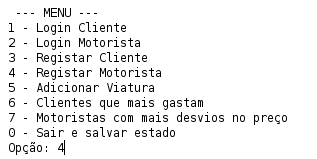
\includegraphics[width=0.5\textwidth]{image4245}
	\caption{\small\sl Menu principal.}
	\captionsetup[figure]{list=yes}
\end{figure}

Escolhendo por exemplo a opção de registar um novo motorista, é-nos apresentado os dados que devemos inserir para registar o novo motorista que após ser registado nos leva de novo ao menu principal.

\begin{figure}[h]
	\centering
	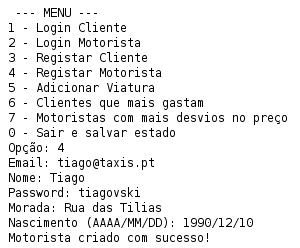
\includegraphics[width=0.5\textwidth]{image4223}
	\caption{\small\sl Registo de um motorista.}
	\captionsetup[figure]{list=yes}
\end{figure}

Por outro lado, escolhendo a opção 1 e inserindo as nossas credenciais somos levados para o menu do cliente. Neste menu podemos ver as nossas informações, ver o nosso relatorio de viagens entre datas e efetuar viagens.

\begin{figure}[h]
	\centering
	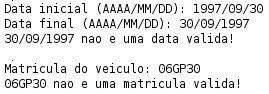
\includegraphics[width=0.45\textwidth]{g4281}
	\caption{\small\sl Formatação das datas e matrículas.}
	\captionsetup[figure]{list=yes}
\end{figure}

Note-se que as datas e as matriculas têm um formato especial e só serão consideradas válidas se respeitarem esse formato.

No menu do motorista (opção 2 no menu principal) é possível ver as nossas informações, ver o nosso relatório de viagens, alterar disponibilidade, mudar de viatura e ver o total faturado pela mesma. 

Temos ainda dados estatísticos nas opções 6 e 7 do menu principal. Estes dados revelam os clientes mais gastadores e os motoristas com maior desvio no preço final.

\begin{figure}[h]
	\centering
	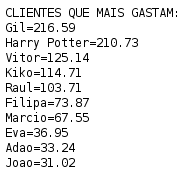
\includegraphics[width=0.3\textwidth]{image4293}
	\caption{\small\sl Clientes mais gastadores.}
	\captionsetup[figure]{list=yes}
\end{figure}

Para sair a opção é o número 0. Esta opção grava o estado da aplicação e quando a volta a iniciar o estado é carregado novamente. A aplicação já tem clientes, motoristas, viaturas e viagens efetuadas para efeitos de teste. As credenciais encontram-se no ficheiro {\sl README.TXT}.

\chapter {Conclusão}

Em geral fazemos um balanço positivo deste trabalho apesar de termos noção de que muitas coisas poderiam ter sido melhoradas se houvesse mais tempo para dedicar.

Entre as coisas que nos deveriamos ter debruçado mais é o facto de não existir uma classe para datas para melhor comparar anos com anos, meses com meses, dias com dias. Assim obteríamos uma melhor organização e controlo.

Um {\sl Array} único de viaturas seria mais vantajoso do que 3 para cada viatura visto que não aproveitamos bem as possibilidade de exploração de cada viatura e acabaram todas por ser bastante similares.

A modularidade na classe {\tt Interface} poderia certamente ser melhorada.

Sentimos também que poderiam ter sido criadas exceções para melhor compreensão de erros que possam eventualmente surgir.

Numa vista abrangente o nosso maior inimigo neste trabalho foi sem dúvida o tempo. Certamente com mais alguns dias de trabalho conseguiríamos por este projeto num nível superior, embora o nível atual seja já satisfatório.
\end{document}